\chapter{Choose Motor}

\section{Motor selection for the mixing tank}
\subsection{Calculate system overall efficiency $ \eta_{sys} $} 
\begin{figure}[ht]
	\centering
	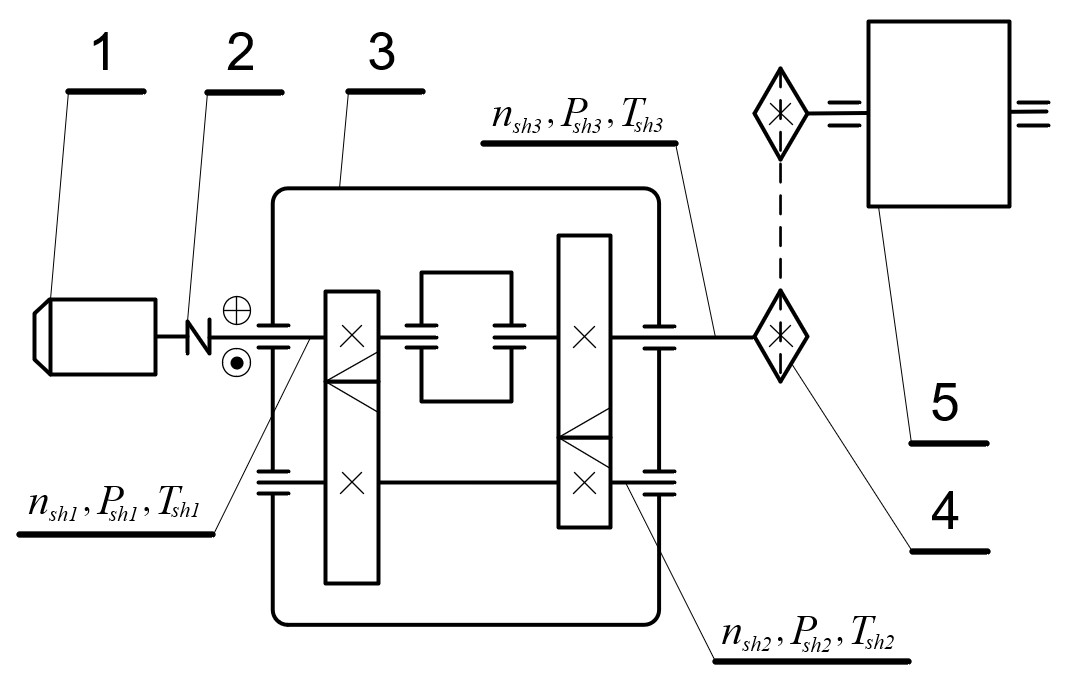
\includegraphics[width=0.75\linewidth]{images/problem2}
	\caption{Working principle diagram with annotation for shafts}
	\label{fig:problem2}
\end{figure}
From Figure \ref{fig:problem2}, the efficiency $ \eta_{sys} $ of the system is calculated using:
\[\eta_{sys} = \eta_c\eta_b^4\eta_{hg}^2\eta_{ch} = 0.99 \times 0.99^4 \times 0.98^2 \times 0.95 = 0.87\]
where
\begin{itemize}
	\item $ \eta_c = 0.99 $ is the flexible coupling efficiency, Table 2.3 \cite{tk1}. The  coupling connects the motor and the speed reducer. In principle, it is designed to transmit torque smoothly while permitting some axial, radial and angular misalignment, typically $ \pm 3^\circ $ \cite{mott_vavrek_wang_2018}. Therefore, the power loss from motor shaft to shaft 1 should be included since it eventually transfers into sound and heat radiation.
	\item $ \eta_b = 0.99 $ is the bearings efficiency, Table 2.3 \cite{tk1}. Housing is provided to 4 rolling bearings, 3 of which are in the speed reducer and the last one is used for the shaft of the mixing tank. During calculations, it is safer to assume the lowest  value for better reliability. Therefore, the lowest efficiency is taken.
	\item $ \eta_{hg} = 0.98 $ is the helical gear efficiency, Table 2.3 \cite{tk1}. In the speed reducer are 2 sealed pairs of helical gear drives. One pair connects shaft 1 and shaft 2, the other connects shaft 2 and 3. A common rule of thumb for spur, helical, and bevel gear meshes is to assume each mesh, including gears and supporting bearings, incurs a 2 percent power loss \cite{collins_busby_staab_2010}.
	\item $ \eta_{ch} = 0.95 $ is the chain drive efficiency, Table 2.3 \cite{tk1}. The chain is protected via housing and provides connection from  the speed reducer to the mixing tank. Similar to the approach from rolling bearing efficiency selection, the efficiency of the chain is chose at the lowest value.
\end{itemize}
\subsection{Calculate required power $ P_{mo} $ for operation} The power $ P $ from design problem is the operating power of the mixing tank. In case of varying load each cycle, the equivalent power $ P_{mo} $ is calculated using  Equation 2.13 \cite{tk1}:
\[P_w = P\sqrt{\dfrac{\left(\dfrac{T_1}{T}\right)^2t_1 + \left(\dfrac{T_2}{T}\right)^2t_2}{t_1+t_2}} = 7 \times \sqrt{\dfrac{\left(\dfrac{T}{T}\right)^2\times15 + \left(\dfrac{0.7T}{T}\right)^2\times11}{15+11}} = 6.2 \unitp{kW}\]
\[P_{mo} = \dfrac{P_w}{\eta_{sys}} = \dfrac{6.2}{0.87} = 7.14 \unitp{kW}\]
where
\begin{itemize}
	\item $ P_w $ is the operating power of the mixing tank given the workload,$ \unit{kW} $.
	\item $ P,T_1,T_2,t_1,t_2$ are given in the design problem; $ \eta_{sys} $ is given in the previous section.
\end{itemize}
%\begin{figure}[ht]
%	\centering
%	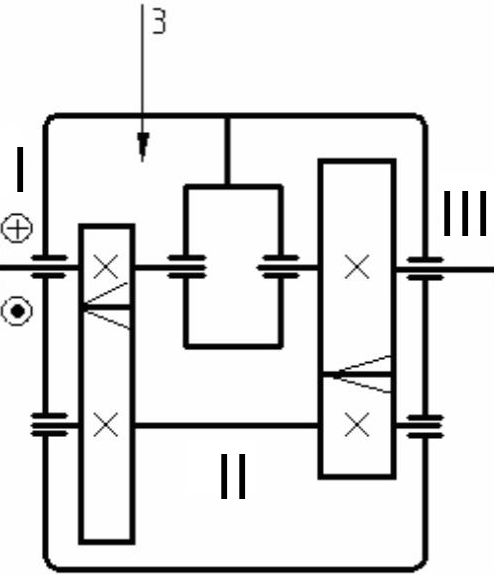
\includegraphics[width=0.35\linewidth]{speed reducer}
%	\caption{Working principle diagram of the speed reducer}
%	\label{fig:speed reducer}
%\end{figure}


\subsection{Choose motor}
There are 2 common speed values for an induction motor in Vietnam which uses line frequency of $ 50\unit{Hz} $:
\begin{enumerate}
	\item Motor with 2 poles at nominal speed $ 3000\unit{rpm} $, which is portable and cheap. However, high system ratio could result in additional expenditure in other machine elements.
	\item Motor with 4 poles at nominal speed $ 1500\unit{rpm} $, which is large and more costly. However, low speed ratio should be adequate since power transmission is the goal of the system, which could in principle, reduce the size of other elements. The choice is this motor type will affect $ u_h $ and $ u_{ch} $ in the next part.
\end{enumerate}

\paragraph{Calculate working speed $ n_{mo} $}
The selection of system speed ratio should be close to $ 1500/n=1500/65= 23.08 $. The working speed $ n_{mo} $ is calculated as:
\[ n_{mo} = u_{sys}n = 22.4 \times 65 = 1456 \unitp{rpm}\]
where
\begin{itemize}
	\item $ u_{sys} $ is the speed ratio of the system. The formula for $ u_{sys} $ is:
	\[ u_{sys} = u_hu_{ch} = 8 \times 2.8 = 22.4\]
	where
	\begin{itemize}
		\item $ u_h = 8 $ is the speed ratio of the speed reducer, which is a 2-level transmission, spur gear type, Table 2.4 \cite{tk1}. The transmission ratio $ u_h $ of the speed reducer should be kept at minimum since in general, it is more costly (material, machining, maintenance, etc.) to manufacture than other mechanical drives such as belt drive and chain drive. The choice of this transmission ratio will be explained clearly in the next section.
		\item $ u_{ch} = 2.8$ is the speed ratio of the chain drive, roller type, Table 2.4 \cite{tk1}. This mechanical drive provides the remaining factor to get close to the desired ratio.
	\end{itemize}
	\item $ n $ is given in the design problem.
\end{itemize}

\paragraph{Choose motor}
%U.S Department of Energy suggests the maximum efficiency of a motor is achieved around $ 75\% $ of the load \cite{department_of_energy_2014}, which in this case is the equivalent load of the system. 
The power of the motor should be around $ P_{mo} = 7.14\unit{kW} $. Thus, from Table P1.3 \cite{tk1}, we choose motor 4A132S4Y3 operating at $ 7.5 \unit{kW} $ maximum and $ 1455 \unit{rpm} $. As a result, the new value for $ n_{mo} $ is $ n_{mo}=1455\unit{rpm} $, which is not much different from $ 1456\unit{rpm} $. Recalculating $ u_{sys} $ with the new $ n_{mo} $:
\[ u_{sys} = n_{mo}/n = 1455/65 = 22.38\]
%\begin{itemize}
%	\item 
%\end{itemize}
Retaining the speed ratio of the speed reducer (i.e. let $ u_h = const = 8 $), the new speed ratio of the chain drive is then:
\[ u_{ch} = u_{sys}/u_h = {22.46}/{8} = 2.83\]

\section{Power, rotational speed and torque of the system}
Let $ P_{sh1} $, $ n_{sh1} $ and $ T_{sh1} $ be the transmitted power, rotational speed and torque onto shaft 1, respectively. Similarly, $ P_{sh2} $, $ n_{sh2} $ and $ T_{sh2} $ are the transmitted parameters onto shaft 2 and $ P_{sh3} $, $ n_{sh3} $ and $ T_{sh3} $ are used for shaft 3. The numbering is specified in Figure \ref{fig:problem2}. Unless otherwise stated, these notations will be used throughout the next chapters.

\subsection{Calculate speed of  the chain drive and the shafts}
\begin{figure}[h]
	\centering
	\begin{subfigure}[t]{.4\linewidth}
		\centering
		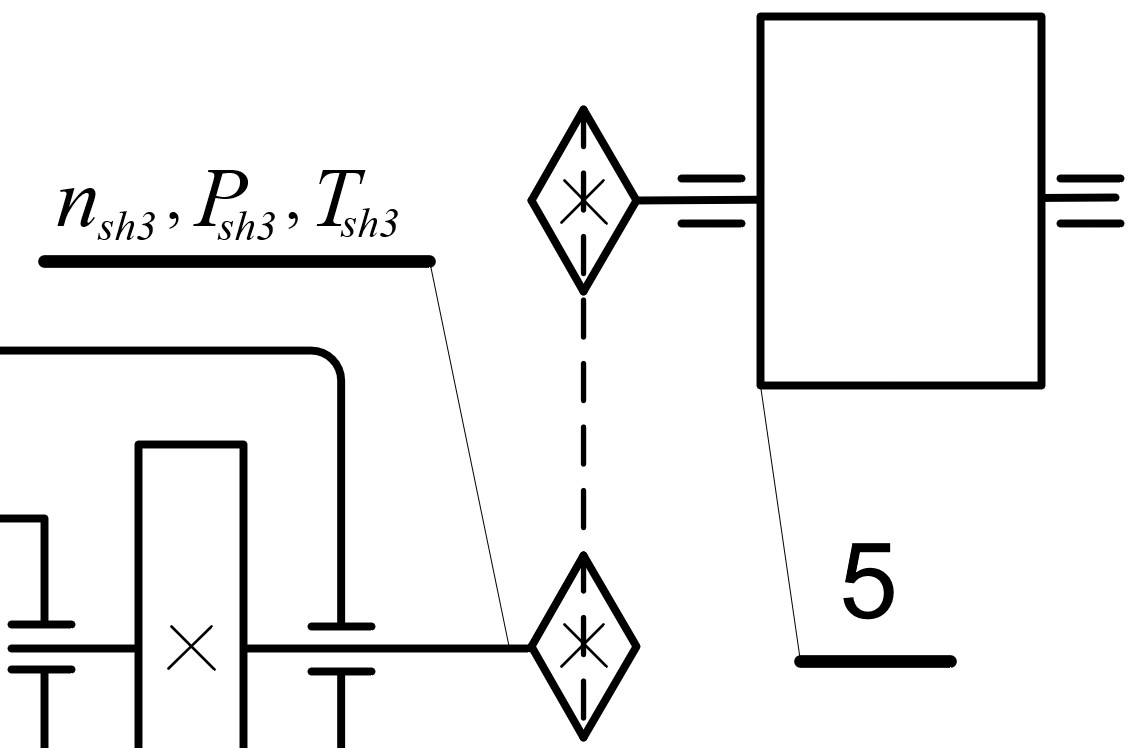
\includegraphics[width=\linewidth,keepaspectratio=true]{p0}
		\caption{Connection between the mixing tank shaft and chain drive: 1 pair of bearings}
		\label{fig:sub1}
	\end{subfigure}\hspace*{0.1\linewidth}
	\begin{subfigure}[t]{.4\linewidth}
		\centering
		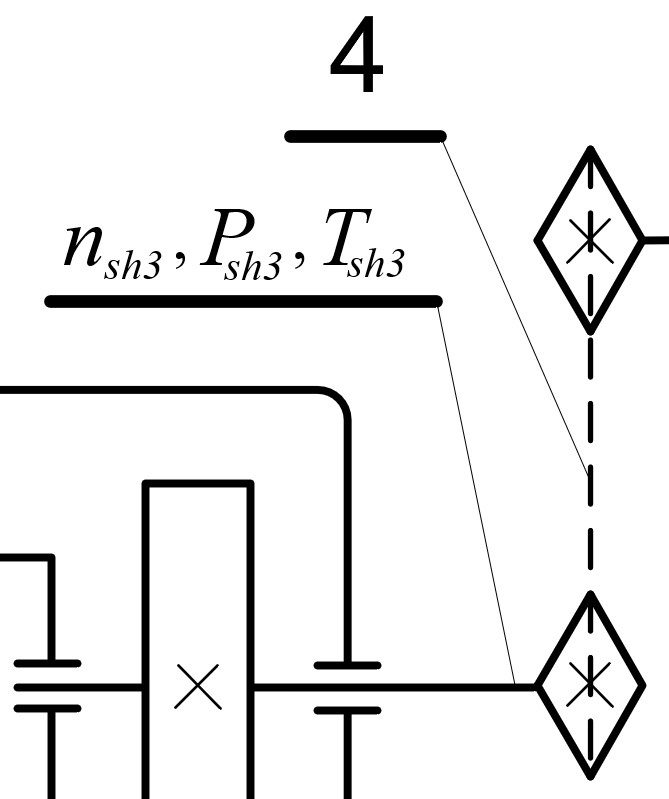
\includegraphics[height=\linewidth,keepaspectratio=true]{p1}
		\caption{Connection between shaft 3 and chain drive: 1 chain drive}
		\label{fig:sub2}
	\end{subfigure}\\
	\begin{subfigure}[t]{.4\linewidth}
		\centering
		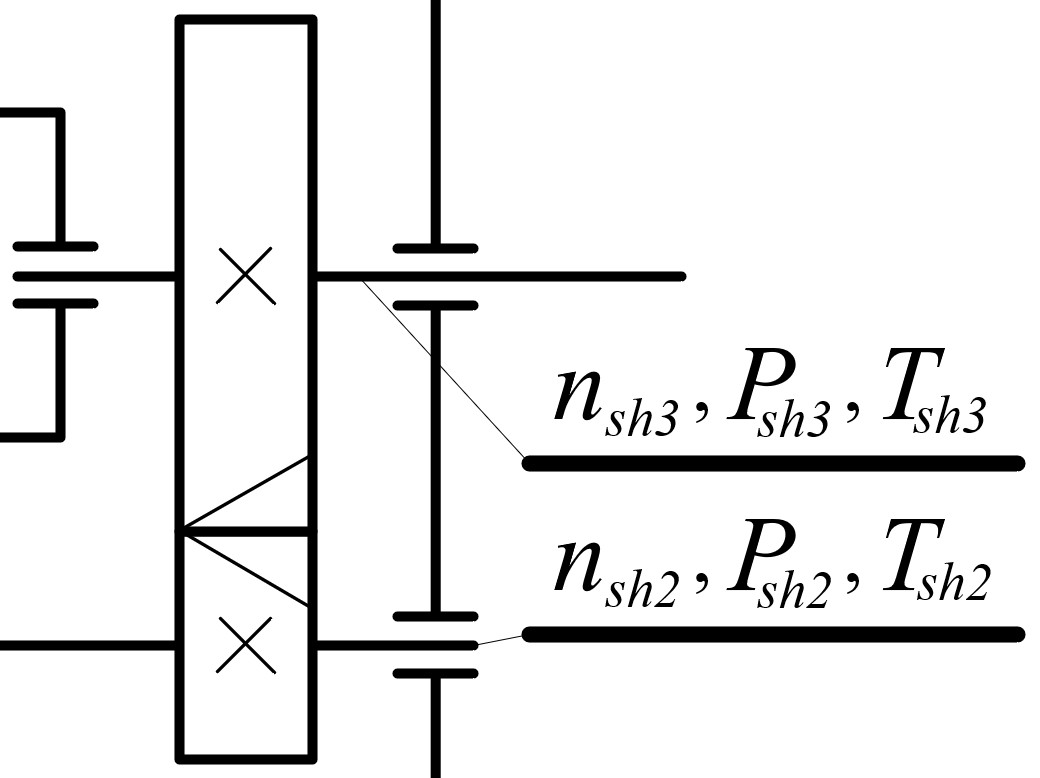
\includegraphics[height=\linewidth,keepaspectratio=true]{p2}
		\caption{Connection between shaft 3 and shaft 2: 1 pair of bearings, 1 spur gear}
		\label{fig:sub3}
	\end{subfigure}\hspace*{0.1\linewidth}	
	\begin{subfigure}[t]{.4\linewidth}
		\centering
		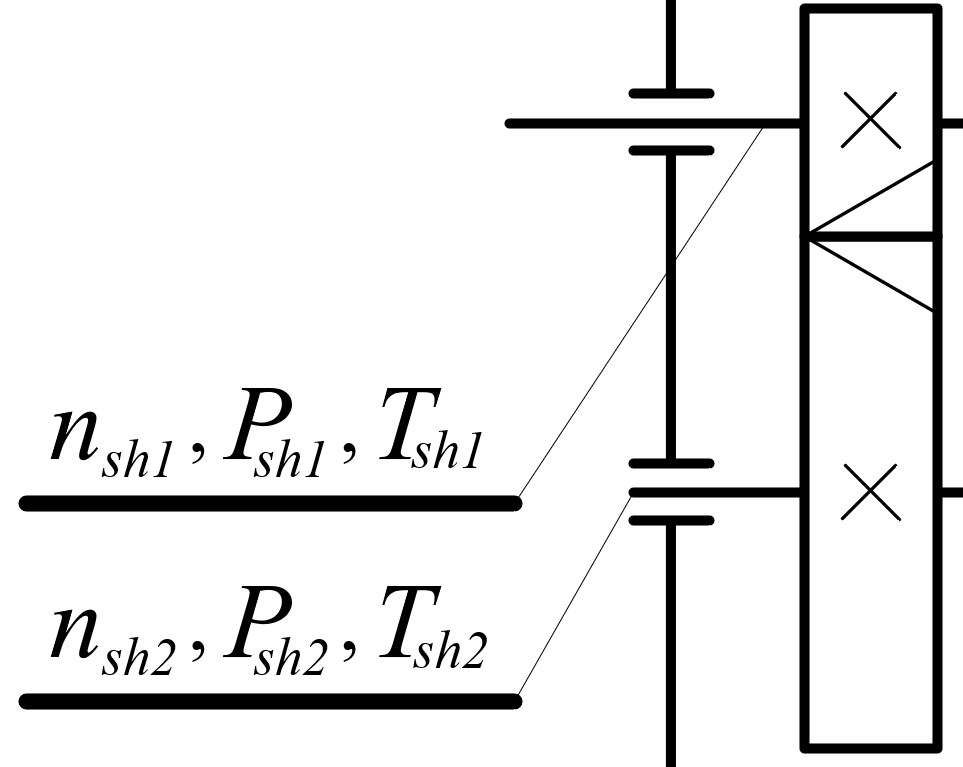
\includegraphics[height=\linewidth,keepaspectratio=true]{p3}
		\caption{Connection between shaft 2 and shaft 1: 1 pair of bearings, 1 spur gear}
		\label{fig:sub4}
	\end{subfigure}
	\caption{Machine elements distribution between shafts and mechanical drives of the system}
	\label{fig:test}
\end{figure}
The entire system is described followed by calculation as follows:\\
Chain drive power $ P_{ch} $ is affected by the bearings on the shaft of the mixing tank:
\[ P_{ch} = \dfrac{P_w}{\eta_b} = \dfrac{6.2}{0.99} = 6.26 \unitp{kW}\]
Shaft 3 power $ P_{sh3} $ is affected by the chain drive:
\[ P_{sh3} = \dfrac{P_{ch}}{\eta_{ch}} = \dfrac{6.26}{0.95} = 6.52 \unitp{kW}\]
Shaft 2 power $ P_{sh2} $ is affected by the bearings and gear drives on shaft 3:
\[ P_{sh2} = \dfrac{P_{sh3}}{\eta_b\eta_{hg}} = \dfrac{6.52}{0.99 \times 0.98} = 6.79 \unitp{kW}\]
Shaft 1 power $ P_{sh1} $ is affected by the bearings and gear drives on shaft 2:
\[ P_{sh1} = \dfrac{P_{sh2}}{\eta_b\eta_{hg}} = \dfrac{6.79}{0.99 \times 0.98} = 7.07 \unitp{kW}\]

\subsection{Calculate speed of the shafts} The design goal of the speed reducer is to lubricate both driven gears equally although there is a size disadvantage. Therefore, the speed ratio of each pair of gears  is calculated using Equation 3.12 \cite{tk1}:
\[u_1=u_2=\sqrt{u_h}=\sqrt{8}=2.83\]
where
\begin{itemize}
	\item $ u_1 $ is the speed ratio of the gear drive attaches to shaft 1 and shaft 2.
	\item $ u_2 $ is the speed ratio of the gear drive attaches to shaft 2 and shaft 3.
\end{itemize}

The value $ u_h $ is chosen deliberately as non-repeating decimal in order to create a \textit{hunting tooth gear set}. A \textit{hunting tooth ratio} is the ratio where the greatest common divisor of the number of teeth in the pinion and driven gear is $ 1 $. Under the same material and surface finishing condition, a greater improvement in the surface roughness was observed in the gears used in the hunting gear ratio compared to non-hunting counterpart even though fatigue damage might be presented. This is especially true for non-finishing soft gears with Brinell hardness number below $ \text{HB}300 $  \cite{Ishibashi1981}.

Then,\\
the speed $ n_{sh1} $ from motor to shaft 1: \[ n_{sh1} = n_{mo} = 1455 \unitp{rpm}\]
the speed $ n_{sh2} $ from shaft 1 to shaft 2: \[ n_{sh2} = {n_{sh1}}/{u_1} = 1455/2.83 = 514.42 \unitp{rpm}\]
the speed $ n_{sh3} $ from shaft 2 to shaft 3: \[ n_{sh3} = {n_{sh2}}/{u_2} = 514.42/2.83 = 181.88 \unitp{rpm}\]

\subsection{Calculate torque of the motor and the shafts}
Subsequently, the torque is calculated as follows:\\
\[ T_{mo}  = 9.55\times10^6 \times P_{mo}/n_{mo} = 9.55\times10^6 \times 7.14/1455 = 46892.66 \unitp{N\cdot mm}\]
\[ T_{sh1} = 9.55\times10^6 \times {P_{sh1}}/{n_{sh1}} = 9.55\times10^6 \times 7.07/1455 = 46423.73 \unitp{N\cdot mm}\]
\[ T_{sh2} = 9.55\times10^6 \times {P_{sh2}}/{n_{sh2}} = 9.55\times10^6 \times 6.79/514.42 = 126093.30 \unitp{N\cdot mm}\]
\[ T_{sh3} = 9.55\times10^6 \times {P_{sh3}}/{n_{sh3}} = 9.55\times10^6 \times 6.52/181.88 = 342486.86 \unitp{N\cdot mm}\]

In summary, we obtain the following table:
\begin{table}[ht]
	\centering
	\caption{Output specification for the shafts and motor}
	\begin{tabular}{lllll}\toprule
		&Motor    & Shaft 1  & Shaft 2  & Shaft 3   \\\midrule
		$ n \unitp{rpm}$ & 1455 & 1455  & 514.42 & 181.88 \\
		$ P \unitp{kW}$ & 7.14  & 7.07   & 6.79   & 6.52   \\
		$ T \unitp{N\cdot mm}$ & 46892.66 & 46423.73 & 126093.30 & 342486.86\\
		$ u $ &       -   &1    &  2.83  & 2.83            \\
		\bottomrule
	\end{tabular}
	\label{tab:my-table}
\end{table}